\documentclass[12pt]{article}
\usepackage[pdftex]{graphicx}

\oddsidemargin  -0.5 cm
\evensidemargin 0.0 cm
\textwidth      6.5in
\headheight     0.0in
\topmargin      -1 cm
\textheight=9.0in
\renewcommand{\arraystretch}{1.5}

\begin{document}

\section*{$\chi_1^+\chi_1^- \to \ell^\pm jj(g)$}

Each chargino decays into a virtual $W^*$ and an LSP neutralino.  We
can read off the chargino-neutralino mass difference from the upper
edge in the $W^*$ mass distribution and determine the neutralino mass
itself from the shape of the $W^*$ lab-frame energy distribution.
Rather than relying on jet algorithms to reconstruct the $W^*$, we can
consider only events where one $W^*$ decays leptonically and the other
hadronically--- this way the total four-momentum in the event, minus
the isolated lepton, is the four-momentum of the $W^*$ (neglecting
lost particles).

Because a muon chamber was not implemented in the detector Monte
Carlo, we could only study $e^\pm jj(g)$ events, but $\mu^\pm jj(g)$
will only add a factor of two to the final yield.  Electrons were
identified as tracks matched to electromagnetic clusters within 10\%
of $E/p = 1$.  These are the rest of the cuts:
\begin{itemize}

  \item Missing energy $>$ 300 GeV (to eliminate most Standard Model
    backgrounds)

  \item Transverse momentum $>$ 15 GeV (to eliminate most
    $\gamma\gamma$ and $e^\pm \gamma$ backgrounds)

  \item Number of tracks $>$ 10 (to make sure that at least one $W^*$
    has decayed hadronically)

  \item Separation angle between electron track and all other tracks
    $>$ 30 degrees

  \item Electron energy $>$ 15 GeV

  \item Electron $|\cos\theta|$ $<$ 0.8 (to cut tagged
    $\gamma\gamma$ and $e^\pm \gamma$ backgrounds)

  \item $W^*$ $|\cos\theta|$ $<$ 0.8 (to cut most Standard Model
    $W^+W^-$)

  \item $W^*$ invariant mass $<$ 70 GeV (to cut the rest of them)

\end{itemize}

\begin{figure}[p]
  \begin{center}
    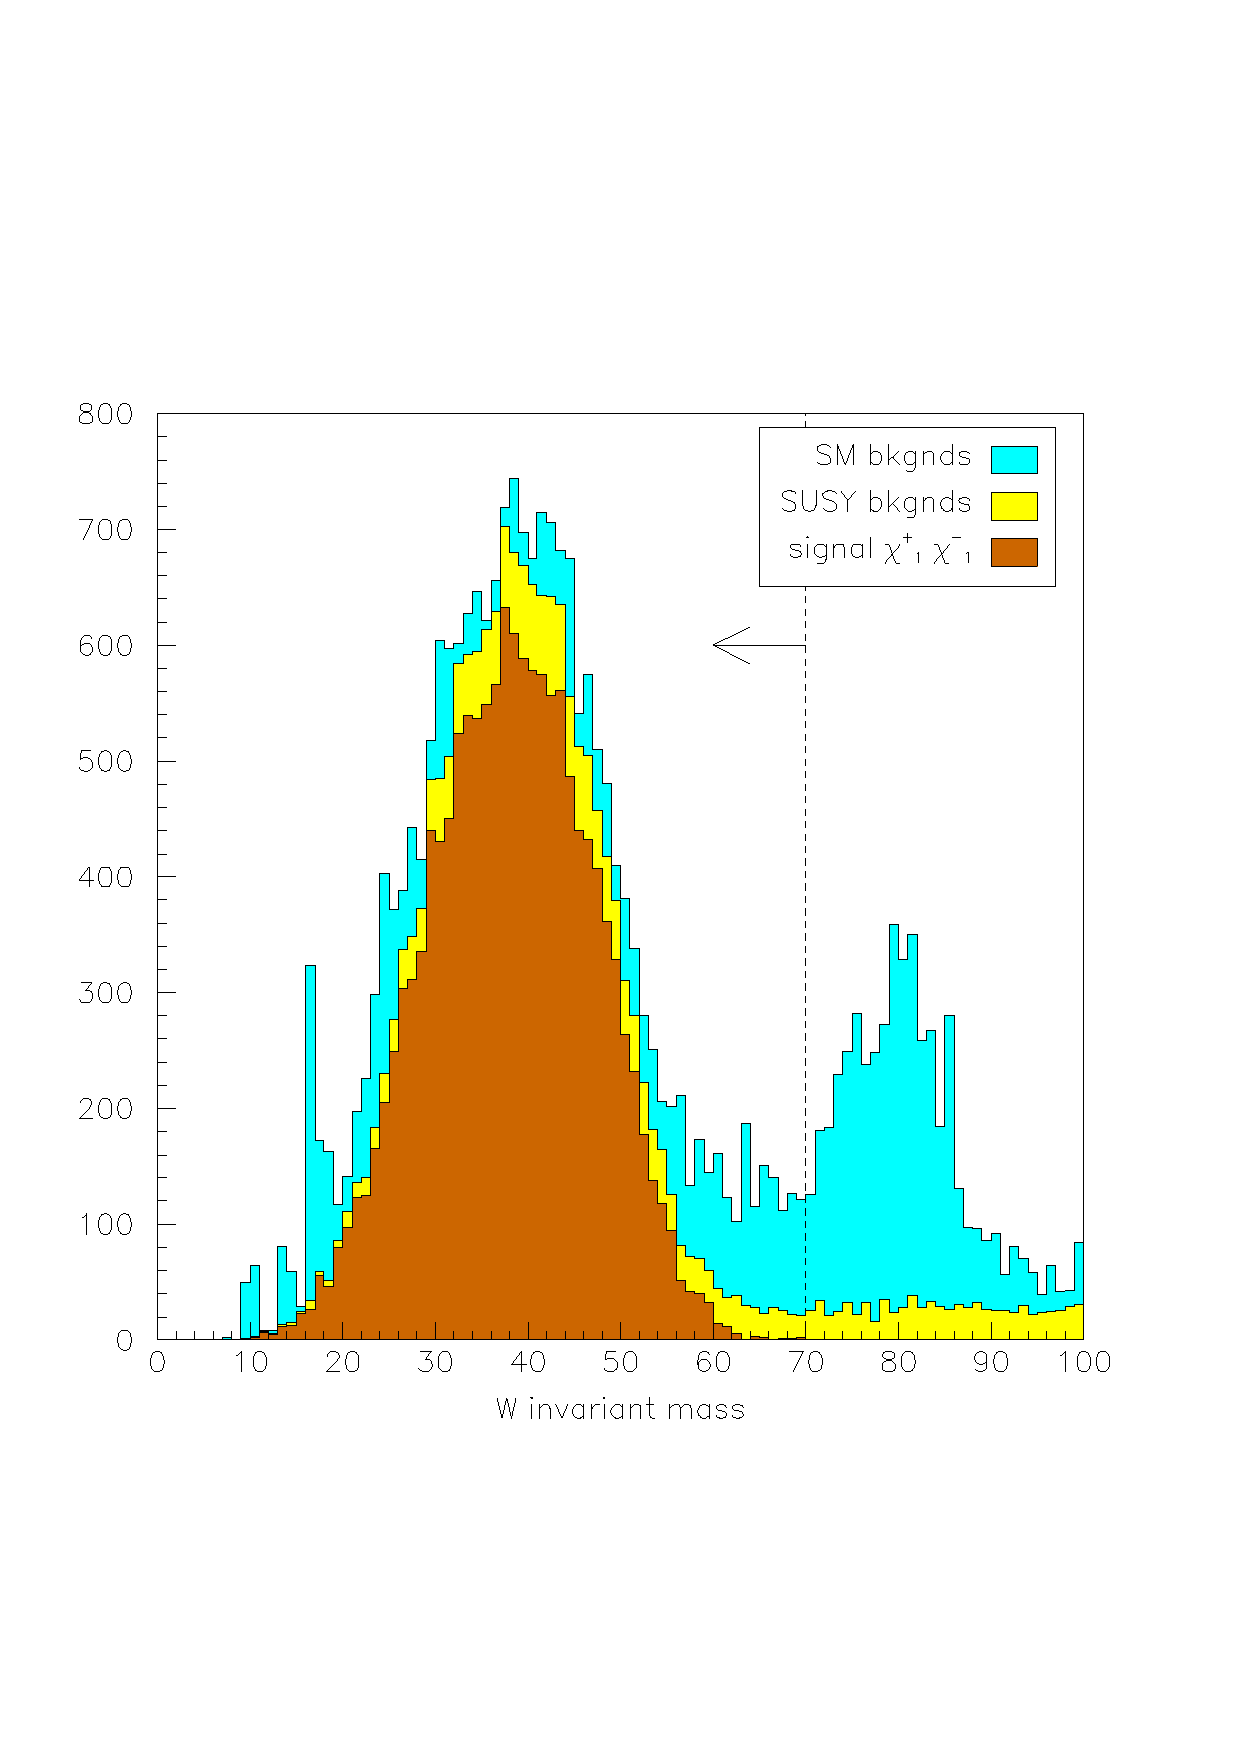
\includegraphics[width=0.7\linewidth]{allnew_8}
  \end{center}

  \caption{The last cut in the $\chi_1^+\chi_1^- \to \ell^\pm jj(g)$
    analysis, showing background contributions stacked on top of the
    signal.  (Both polarizations are combined.) \label{jimp_cutplot}}
\end{figure}

\begin{table}[p]
  \begin{center}
    \begin{tabular}{l c c}
      & left-pol. & right-pol. \\
      Signal ($\chi_1^+\chi_1^- \to e^\pm jj(g)$) & 12421 & 1592 \\
      SUSY backgrounds (including $\chi_1^+\chi_1^-$ to other modes) & 1751 & 480 \\
      Standard Model backgrounds & 3170 & 1209 \\\hline
      Cross-section measurement & 940 $\pm$ 10 fb & 119 $\pm$ 4.3 fb
    \end{tabular}
  \end{center}

  \caption{The signal and background yields for both incident-electron
    polarizations and the uncertainty on the cross-section
    measurement.  The uncertainties can be reduced by a factor of
    $\sqrt{2}$ if the $\mu^\pm jj(g)$ mode is also included.
    ($\mu^\pm jj(g)$ is not a significant contribution to the SUSY
    backgrounds.) \label{jimp_table}}
\end{table}

The branching fraction for $\chi_1^+\chi_1^- \to e^\pm jj(g)$ is 15\%
(entirely dominated by the leptonic and hadronic $W$ branching
fractions), and the efficiency for such a final state to pass the
above cuts is 36\%.  The branching fractions and efficiencies do not
depend on the polarity of the incident beams, but because
$\chi_1^+\chi_1^-$ production prefers left-handed electrons by a ratio
of 8:1, the final yields do.  The yields and backgrounds are listed in
Table \ref{jimp_table} and the last cut is plotted in Figure
\ref{jimp_cutplot}.  Despite the preference for left-handed
production, it is still favorable to combine the left-handed and
right-handed datasets for a 1\% cross-section measurement, after
background subtraction.  (This 1\% is further reduced by a factor of
$\sqrt{2}$ if the $\mu^\pm jj(g)$ mode is included.)

\begin{figure}[t]
  \begin{center}
    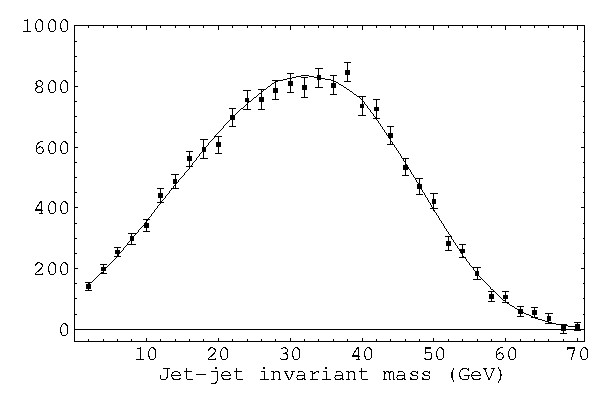
\includegraphics[width=0.47\linewidth]{fake3_mass} \hfill
    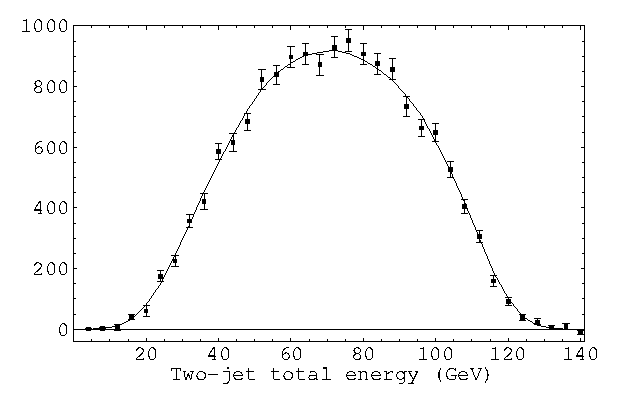
\includegraphics[width=0.47\linewidth]{fake3_energy}
  \end{center}

  \caption{Projections of the 2-D $W^*$ invariant mass/lab-frame
    energy distribution, overlaid on mock background-subtracted
    data.  ($\zeta$ was chosen to be 0.9.) \label{jimp_wmassenergy}}
\end{figure}

The chargino-neutralino mass difference could be read off the $W^*$
invariant mass plot (Figure \ref{jimp_cutplot}) if it were not blurred
by detector resolution.  Even if this wasn't a problem, the dependence
of the absolute neutralino mass on the $W^*$ lab-frame energy is far
from simple, so some kind of fitting procedure must be applied to both
distributions to extract the masses.  We implemented a fitter which
assumes a neutralino mass, a chargino mass, and a [vector-axial?]
parameter $\zeta$ to generate 2-D distributions of the $W^*$ invariant
mass and lab-frame energy, which can then be fit to the data.  The
$W^*$ mass is generated using [Andreas's distribution], and its energy
is derived from energy conservation, accounting for energy lost to
initial state radiation and beamstrahlung and the neutralinos.
Naturally, the beam energy loss needs to be understood very well to
apply this procedure in a realistic environment.  To approximate
detector effects, the $W^*$ invariant mass is convolved with a 8.4 GeV
Gaussian and the $W^*$ lab-frame energy is independently convolved
with a 6.0 GeV Gaussian.  These resolutions and their independence
were derived by comparing the measured $W^*$ mass and energy with
their generator values in the Monte Carlo.

In this fitting example, the statistical errors on the data are the
square root of the number of events left after cuts, inflated by
background subtraction.  Because it would slow down the fitting
procedure, event cuts were not simulated in the fitter.  The event
cuts sculpt the shape of the energy and mass distributions, so the
``data'' distribution to which we fitted was actually generated by the
fitter: it is a no-cuts distribution with na\"ive resolution.  All
these effects left out of the fitter can bias the final fit, so this
study is completely insensitive to any systematic errors that would
plague a real experiment.  These uncertainty predictions, therefore,
must be understood as purely statistical.  Projections of the
generated distribution overlaid on the nominal fit are shown in Figure
\ref{jimp_wmassenergy}.

\begin{figure}[p]
  \begin{center}
    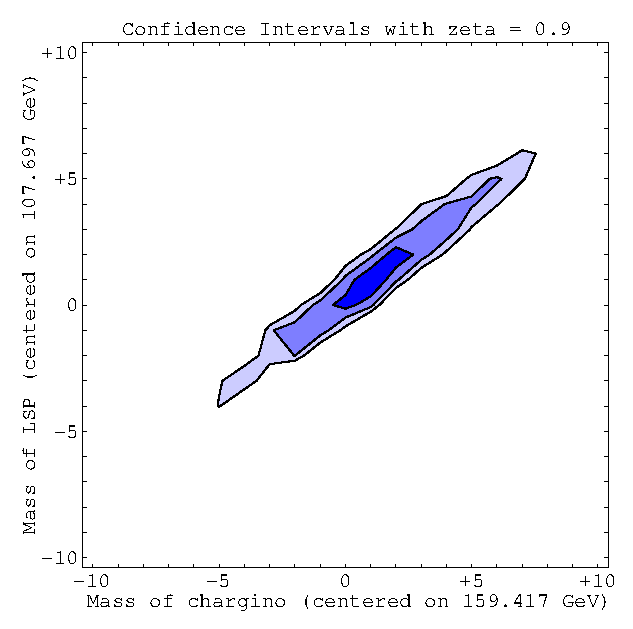
\includegraphics[width=0.7\linewidth]{fake3_contours}
  \end{center}

  \caption{One-, two-, and three-sigma contours in chargino and
    neutralino mass with $\zeta$ = 0.9.  This plot is centered on the
    input mass values and is gradated in units of
    GeV. \label{jimp_contours}}
\end{figure}

\begin{table}[p]
  \begin{center}
    \begin{tabular}{l c}
      LSP neutralino mass ($m_{\chi_1^0}$) & $\pm$1.1 GeV \\
      chargino mass ($m_{\chi_1^\pm}$) & $\pm$1.9 GeV \\
      mass difference ($m_{\chi_1^\pm} - m_{\chi_1^0}$) & $\pm$0.4 GeV \\
      mass sum ($m_{\chi_1^\pm} + m_{\chi_1^0}$) & $\pm$1.8 GeV \\
      $\zeta$ (vector-axial thingy, set to 0.9) & $\pm$0.012 \\
    \end{tabular}
  \end{center}

  \caption{Sensitivities to and correlations between chargino and
      neutralino masses.  ($\zeta$ was fit independently of
      $m_{\chi_1^0}$ and $m_{\chi_1^\pm}$.) \label{jimp_errors}}
\end{table}

The results of this fit are shown in Figure \ref{jimp_contours} and
Table \ref{jimp_errors}.  Because the upper edge of the mass
distribution is sensitive to the mass difference, the difference is
much better constrained than either mass.  $\zeta$ dramatically widens
the shape of the invariant mass distribution, so it is very well
constrained, but it doesn't interfere with the location of the upper
edge, so it can be fitted independently.

\end{document}
